\chapter{Métodos Iterativos}
Como ya hemos visto, los métodos directos poseen en general una complejidad de orden cúbico en el número de incógnitas $\mathcal{O}(N^3)$. Esto dice que si en un problema determinado se duplica el número de incógnitas entonces el número de operaciones se multiplica por 8. Eso ha llevado a intentar desarrollar métodos de orden menor \footnote{Observe que el límite inferior para un método de resolución  es $\mathcal{O}(N^2)$ ya que ese es el número de coeficientes de la matriz.} y los métodos iterativos son una posible alternativa.

Hay, además de la complejidad,  otros problemas con los métodos directos. Por ejemplo, en muchas aplicaciones aparecen problemas con un número muy grande de incógnitas pero con matrices \emph{ralas}, es decir, matrices con un elevado porcentaje de coeficiente nulos. Esto permite en principio reducir notablemente el número de operaciones del algoritmo pero sin embargo como desventaja aparece un ``rellenado'' innecesario en la factorización resultante. En la siguiente sección vemos un ejemplo sencillo.

\section{Un ejemplo: distribución de temperatura}
\label{sec:piston}
Ciertas ecuaciones diferenciales lineales  pueden resolverse de modo aproximado a través de \emph{discretizaciones}.
En dimensión uno es fácil imaginar como puede hacerse. Por ejemplo, consideremos en el intervalo $[a,b]$ la ecuación diferencial
\begin{equation}
 \label{eq:calor1d}
\left\lbrace
\begin{matrix}
u''(x)&=f(x),\\
u(a)&=0,\\
u(b)&=0.
\end{matrix}
\right.
\end{equation}

Aquí, $f(x)$ representa un dato conocido. Podemos aproximar el problema en dimensión finita del siguiente modo: consideramos puntos (en este ejemplo uniformemente distribuidos) $a=x_0<x_1<\cdots <x_{n+1}=b$ tales que $x_i=a+ih$ donde $h=\frac{b-a}{n+1}$.  Cuando $n\to \infty$ (aumentamos el número de puntos) resulta que $h\to 0$ y como
$$
\frac{u(x_{i+1})-2u(x_i)+u(x_{i-1})}{h^2}=
\frac{u(x_{i}+h)-2u(x_i)+u(x_{i}-h)}{h^2}
$$
tenemos para $u$ suficientemente derivable
$$
u(x_{i}+h)=u(x_{i})+u'(x_i)h+u''(x_i)h^2/2+u'''(x_i)h^3/3!+\mathcal{O}(h^4)
$$
$$
u(x_{i}-h)=u(x_{i})-u'(x_i)h+u''(x_i)h^2/2-u'''(x_i)h^3/3!+\mathcal{O}(h^4)
$$
y así
$$
\frac{u(x_{i}+h)-2u(x_i)+u(x_{i}-h)}{h^2}=u''(x_i)+\mathcal{O}(h^2),
$$
por lo que usando que $u''(x_i)=f(x_i)$, vemos que podemos aproximar la temperatura en el punto $x_i$ resolviendo
$$
u(x_{i+1})-2u(x_i)+u(x_{i-1})=f(x_i)h^2,
$$
lo que conduce a un sistema \emph{tridiagonal y simétrico}, con una ecuación por cada $x_i$,  que se escribe\footnote{$u(x_0)=u(x_{n+1})=0$ no son incógnitas del sistema, por ello no están en la ecuación.}
\begin{equation}
\label{eq:unid}
\begin{pmatrix}
-2&1&0&0&\cdots &0&0\\
1&-2&1&0&\cdots &0&0\\
0&1&-2&1&\cdots &0&0 \\
\vdots&\vdots&\vdots&\vdots&
\cdots &\vdots&\vdots\\
0&0&0&0&\cdots& 1&-2
\end{pmatrix}
\begin{pmatrix}
 u(x_1)\\
 u(x_2)\\
 \vdots\\
 u(x_n)
 \end{pmatrix}=h^2
 \begin{pmatrix}
 f(x_1)\\
 f(x_2)\\
 \vdots\\
 f(x_n)
 \end{pmatrix}.
\end{equation}
La ecuación \eqref{eq:calor1d} modeliza (en un caso muy elemental y sin contemplar constantes físicas) el problema de la distribución de temperatura en una barra unidimensional. En dimensión mas alta (por ejemplo en dimensión 3) el problema se puede modelizar con la  ecuación\footnote{Recordar que $\Delta$ representa al Laplaciano de $u$. En dimensión 3 por ejemplo se escribe $\Delta u=u_{xx}+u_{yy}+u_{zz}$.}
$$
\Delta u(x)=f(x).
$$
Para ver un ejemplo concreto en la Figura \ref{fig:disc_piston} se muestra un cuarto de pistón (pieza que se desplaza dentro de uno de los cilindros de un motor). La distribución de temperatura en esa pieza puede aproximarse como antes  través de una discretización.
\begin{figure}[h]
\centering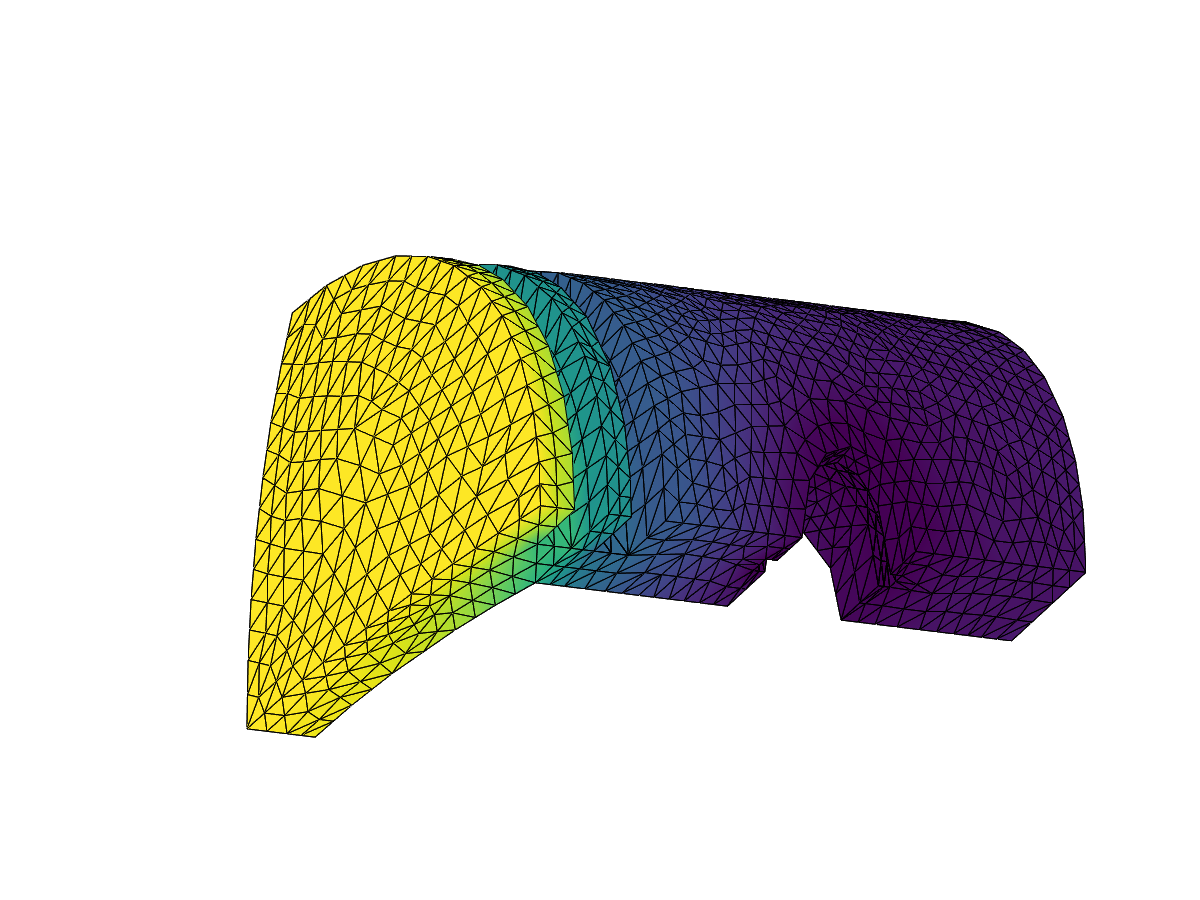
\includegraphics[width=0.3\linewidth]{piston.png}
\label{fig:disc_piston}
\caption{Distribución de temperatura en un pistón. Se visualiza un cuarto de la pieza.}
\end{figure}
No vamos a describir aquí como hacer esto, pero una vez discretizado, el problema puede escribirse, al igual que el problema unidimensional, como un sistema lineal de ecuaciones. En este ejemplo particular, se obtiene un sistema
 $$
 \Ab\xb=\bb,
 $$

 $$\Ab\in \R^{3319\times 3319}$$
donde cada incógnita es el valor de la temperatura en un punto interior del pistón. Este ejemplo (que llamaremos $(E)$ ) nos servirá para ejemplificar algunas particularidades que aparecen en este capítulo. Si bien esta matriz $\Ab$ no es mas tridiagonal \emph{sí es simétrica}, además de  rala\footnote{ En inglés sparse: un porcentaje significativo de elementos de la matriz es nulo.}. En la Figura \ref{fig:matrizA}
\begin{figure}[h]
\label{fig:matrizA}
\centering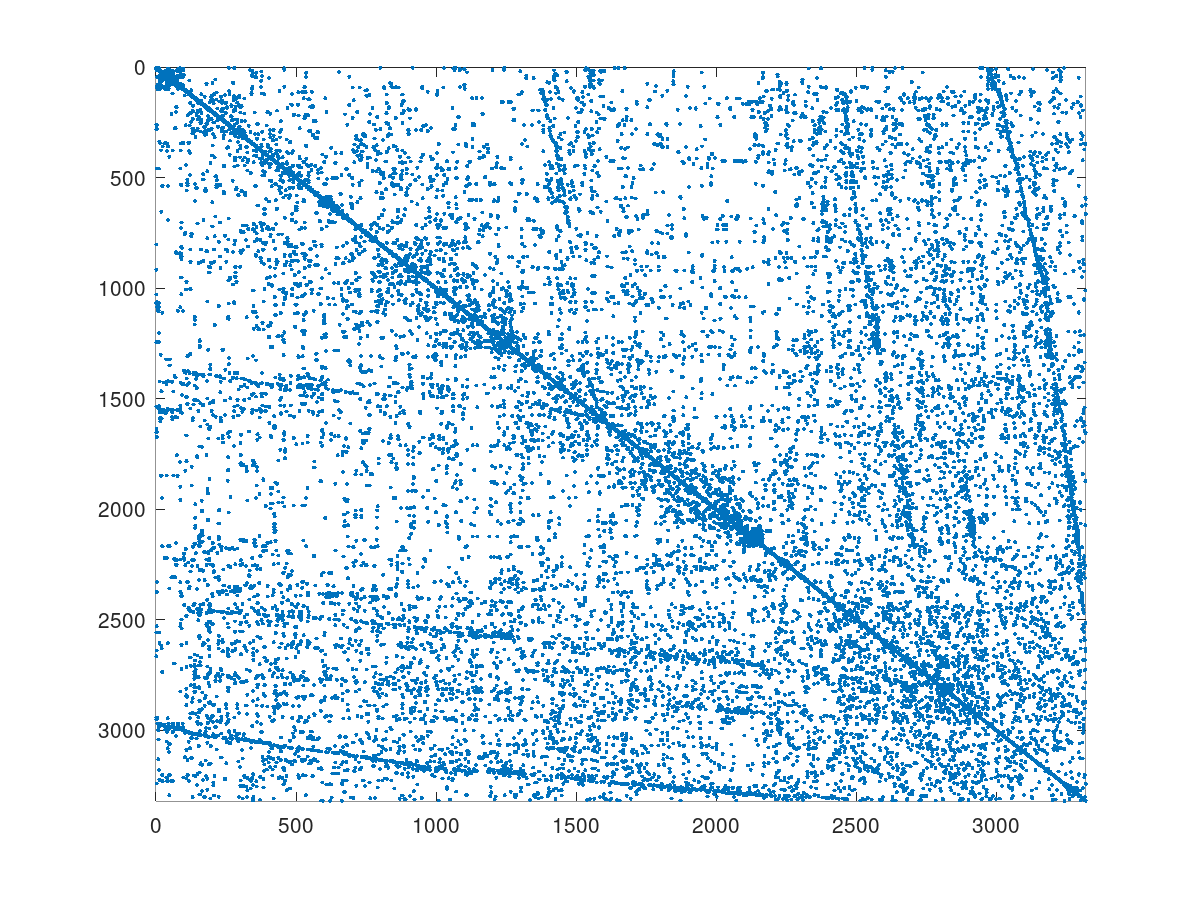
\includegraphics[width=0.4\linewidth]{matrizA.png}
\caption{Estructura de la matriz $A$: se observa que es rala y simétrica.}
\end{figure}
se observan ambos hechos (con el comando np.spy(A)). En este caso, solamente $39753$ coeficientes son diferentes de cero, en vez $3319^2=11015761$ que representan el total de elementos de la matriz. Desde  el punto de vista de la memoria utilizada en el almacenamiento de $\Ab$ esto es significativo. Teniendo en cuenta que en doble precisión cada número ocupa 8 bytes tendriamos en cada caso:
\begin{itemize}
 \item $39753\frac{8}{1024}\sim 300K$
 \item $11015761 \frac{8}{(1024)^2}\sim 84M$.
\end{itemize}
Esta ventaja se puede perder al hacer $LU$.
En efecto, en este ejemplo, a pesar de que $A$ tiene solo $39753$ elementos no nulos, el número de elementos no nulos de $L$ es $2440542$ ($\sim 18M$). Este fenómeno se conoce como \emph{rellenado}. La apariencia de $L$ y su comparación con la matriz original puede verse en la Figura \ref{fig:LyA}

\begin{figure}[h]
\centering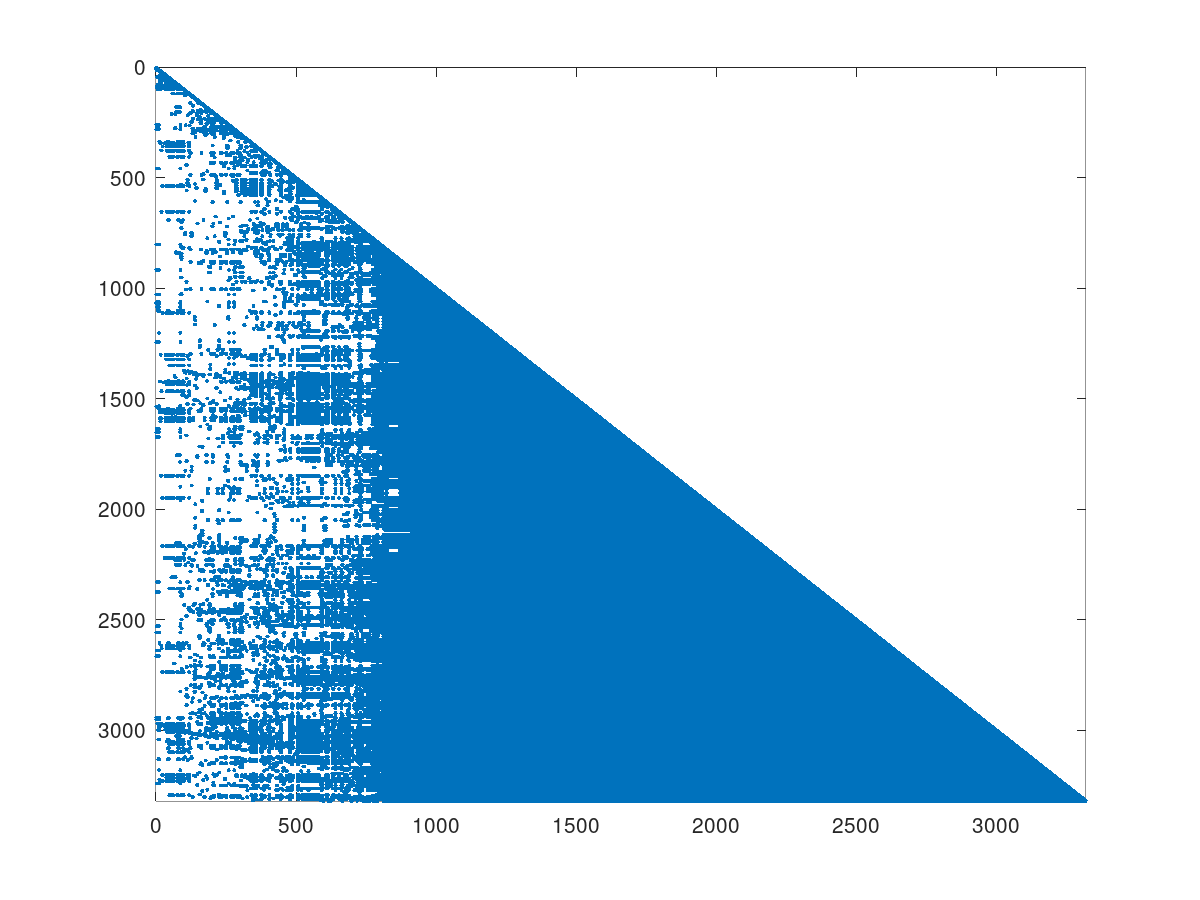
\includegraphics[width=0.3\linewidth]{matrizL.png}
\centering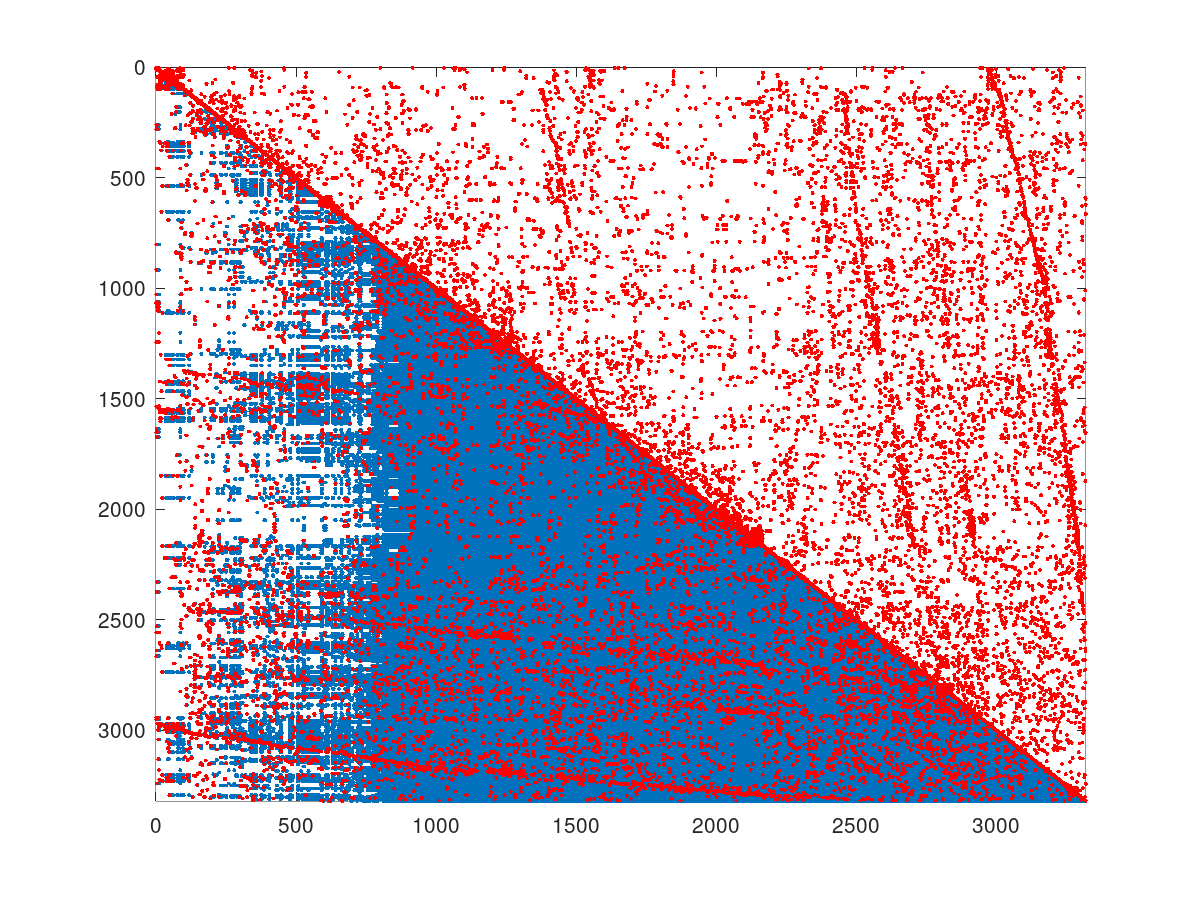
\includegraphics[width=0.3\linewidth]{matricesAyL.png}
\label{fig:LyA}
\caption{Estructura de las matrices $A$ y $L$ en el ejemplo $(E)$. Izquierda, matriz $L$ de la factorización $A=LU$ donde se nota el rellenado. Derecha, superposición de $A$ y $L$.}
\end{figure}


Si bien hay heurísticas para evitar el rellenado, buscando permutar las variables y las ecuaciones no las vamos a comentar en este texto. Vamos a concentrarnos en los métodos iterativos. Estos no buscan ninguna factorización y se basan en iterar un procedimiento de orden $\mathcal{O}(N^2)$ (básicamente el producto de una matriz por vector)  con el esperanza de conseguir una buena aproximación de la solución buscada en unas pocas \footnote{Pocas al menos relativo al tamaño $N$ de la matriz.} iteraciones.

Ya hemos visto que $\rho(\Ab)$ no es una norma, sin embargo verifica:
$$
\rho(\Ab)=\inf_{\|\cdot\|} \|\Ab\|.
$$
Lo que implica que para todo $0<\varepsilon$ existe una norma $\|\cdot\|$ tal que
$$\|\Ab\|\le \rho(\Ab)+ \varepsilon$$ Usaremos esta propiedad en la demostración del siguiente resultado que da la clave para predecir el orden de convergencia de los métodos iterativos.
\tcc
\begin{prop}
 Para toda norma subordinada $\|\cdot\|$ vale que
 $$
 \rho(\Mb)=\lim_{k\to \infty} \|\Mb^k\|^{1/k}.
 $$
\end{prop}

\etcc


\begin{proof}
 Dado $\epsilon>0$ existe una norma subordinada $\|\cdot\|_{*}$ tal que
 $$
 \|\Mb\|_{*}\le \rho(\Mb)+\epsilon.
 $$
 $$
 \rho(\Mb)^k=\rho(\Mb^k)\le \|\Mb^k\|\le C \|\Mb^k\|_{*}\le C \|\Mb\|^k_{*}\le C(\rho(\Mb)+\epsilon)^k,
 $$
 $$
 \rho(\Mb)\le \|\Mb^k\|^{1/k}\le C^{1/k}(\rho(\Mb)+\epsilon)
 $$
 tomando límite y notando que $\epsilon$ es arbitrario se demuestra el resultado.
\end{proof}
\section{Métodos Iterativos}
Supongamos que queremos resolver
$$
\Ab\xb=\bb,
$$
pero la matriz $\Ab$ es difícil de invertir. Entonces proponemos una descomposición
$$\Ab=\Bb+\Cb,$$
donde $\Bb$ es elegida de modo que sea \emph{fácil} de invertir y escribimos
$$
\Bb\xb=-\Cb\xb+\bb,
$$
o equivalentemente
$$
\xb=-\Bb^{-1}\Cb\xb+\Bb^{-1}\bb.
$$
Notemos que llamando $\Mb_I=-\Bb^{-1}\Cb$  (denominada \emph{matriz de iteraciones}) y $\Bb^{-1}\bb=\tilde{\bb}$,  resolver el sistema equivale a hallar $\xb$ tal que
$$
\xb=\Mb_I\xb+\tilde{\bb}.
$$
La idea es tomar un vector inicial $\xb_0$ e iterar
$$
\xb_{n+1}=\Mb_I\xb_n+\tilde{\bb},
$$
con la esperanza de que $\xb_k\to \xb$. Para ver si nuestra idea puede funcionar estudiamos el error $\eb_k=\xb-\xb_k$ restando miembro a miembro las dos ecuaciones de arriba
$$
\eb_{k+1}=\Mb_I\eb_k=\Mb_I\Mb_I\eb_{k-1}=\cdots = \Mb^{k+1}_I\eb_0
$$
de donde vemos que $\eb_k\to \cero$ para \emph{todo} error inicial $\eb_0$ sí y solo sí
$\Mb_I^{k}\to \cero $ lo cual ocurre sí y solo sí $\rho(\Mb_I)<1$.

Más aún
$$
\|\eb_k\|\le C\rho(\Mb_I)^k
$$
lo que nos da la velocidad de convergencia del algoritmo.

Comencemos estudiando un caso particular llamado el método de Richardson.
 Elegimos $\Bb$ como un múltiplo de la identidad
$$\Bb=\omega^{-1}\Ib, \qquad \omega>0.$$
Luego, se tiene
$$\Cb=\Ab-\omega^{-1}\Ib=\omega^{-1}(\omega\Ab-\Ib)$$
y la matriz de iteraciones resulta
$$
\Mb_I=-\Bb^{-1}\Cb=
\Ib-\omega\Ab
$$

\tcc
\begin{prop}
Si $\Ab$ es SDP, el método de Richardson converge -para todo dato inicial- sí y solo sí $\omega<\frac{2}{\rho(\Ab)}.$
\end{prop}
\etcc

\begin{proof}
 Basta ver bajo que condiciones $\rho(\Mb_I)<1$, con $
\Mb_I=
\Ib-\omega\Ab.
$ Como $\Ab$ es SDP sus autovalores cumplen $0<\lambda_1\le \lambda_2\le \cdots \le \lambda_n$. Los autovalores de $
\Mb_I$ son entonces $1-\omega\lambda_i$.  Queremos ver bajo que condiciones
$
|1-\omega\lambda_i|<1,
$ para todo $1\le i\le n$. Equivalentemente,
$$
-1< 1-\omega\lambda_i< 1
$$
i.e. es necesario y suficiente que $\omega<\frac{2}{\lambda_i}$ para todo $1\le i\le n$ lo que equivale a
$\omega<\frac{2}{\rho(\Ab)}.$
\end{proof}

Claramente, al variar $\omega$ en el rango $(0,\frac{2}{\rho(\Ab)})$ obtendremos distintas velocidades de convergencia para nuestro método. Podemos intentar localizar el óptimo $\omega_{opt}$, es decir el que garantiza orden máximo de convergencia (equivalentemente, el $\omega_{opt}$ para el cual $\rho(\Mb_I)$ es mínimo). Para ello observemos que   (ver Figura \ref{fig:modulos}) como
$$
\rho(\Mb_I)=\max\{
|1-\omega   \lambda_n|,|1-\omega   \lambda_1|\}
$$
$\omega_{opt}$ ocurre en el punto de cruce de los gráficos.
\begin{figure}[h]
\label{fig:modulos}
\centering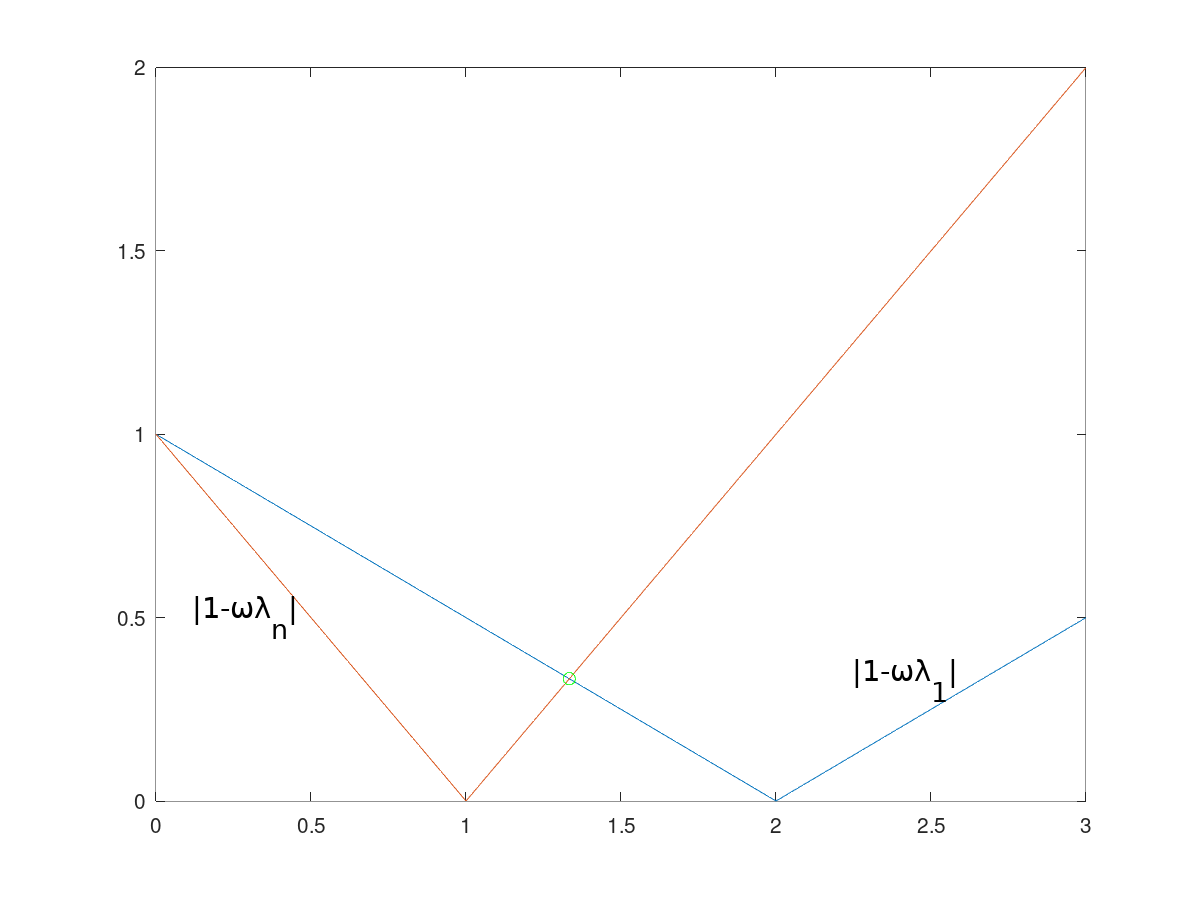
\includegraphics[width=0.4\linewidth]{modulos.png}
\end{figure}
Ese punto puede despejarse
$$
\omega_{opt}=\frac{2}{\lambda_n+\lambda_1}
$$
de donde el respectivo radio espectral óptimo es
$$\rho(\Mb_I)=\frac{\lambda_n-\lambda_1}{\lambda_n+\lambda_1}=\frac{\kappa(\Ab)-1}{\kappa(\Ab)+1}.
$$
Notemos que la velocidad de convergencia del método se deteriora si  $\kappa(\Ab)$ es grande.

\tcc
Para el ejemplo $(E)$ de la distribución de temperatura, dado al principio del capítulo, tenemos (aproximados por el método de la potencia)

$$
\lambda_1\sim 0.0009 \qquad \lambda_n \sim 1.93
$$

$$\kappa(\Ab)\sim 2144$$

$$\omega_{opt}\sim
1.04$$
lo que da
$$\rho(\Mb_I)\sim 0.99907$$
si queremos reducir  el error inicial en un orden  de $10^{-3}$ precisamos iterar aproximadamente $60000$ veces, número mucho mayor que el tamaño  $n\sim 3000$ de la matriz. Como vemos no resulta muy competitivo en este caso.
\etcc


\section{Algunos Métodos Clásicos}



Si tomamos $\Ab=\Lb+\Db+\Ub$ (triangular inferior+diagonal+triangular superior), podemos ensayar varias descomposiciones $\Ab=\Bb+\Cb$:
\begin{enumerate}
 \item $\Bb=\Db$ método de Jacobi
 \item $\Bb=\Lb+\Db$ método de Gauss-Seidel
\end{enumerate}

Las matrices de iteración son
\begin{enumerate}
 \item Jacobi $\Mb_J=-\Db^{-1}(\Lb+\Ub)$
 \item Gauss-Seidel $\Mb_{GS}=-(\Lb+\Db)^{-1}\Ub$
\end{enumerate}

Si bien en el caso GS, contrariamente al  caso J, la matriz no parece obviamente invertible, originalmente fueron concebidos del  modo siguiente que no requiere inversiones explícitas:
de
$$
\Ab\xb=\bb,
$$
se tiene, para todo $1\le i\le n$
$$
\sum_{j=1}^na_{i,j}x_j=b_i,
$$
en Jacobi se escribe (asumiendo $a_{i,i}\neq0$)
$$
x_i=\left(-\sum_{j=1,j\neq i}^na_{i,j}x_j+b_i\right)/a_{i,i}\, \qquad \forall 1\le i\le n
$$
que da lugar al método
$$
x_i^{(k+1)}=\left(-\sum_{j=1,j\neq i}^na_{i,j}x_j^{(k)}+b_i\right)/a_{i,i}\, \qquad \forall 1\le i\le n
$$
para pasar del iterado $k$ al $k+1$.



Para Gauss-Seidel se escribe
$$
x_i^{(k+1)}=\left(-\sum_{j=i+1}^na_{i,j}x_j^{(k
)}-\sum_{j=1}^{i-1}a_{i,j}x_j^{(k+1)}+b_i\right)/a_{i,i}\, \qquad \forall 1\le i\le n
$$
para pasar del iterado $k$ al $k+1$, con la idea de  utilizar
$x_1^{(k+1)},\cdots x_{i-1}^{(k+1)}$ (considerados \emph{mejores} aproximaciones) en el cálculo de $x_i^{(k+1)}$.

Notar que:
\begin{itemize}
\item No es necesiario construir explícitamente $M_J$ no $M_{GS}$.
 \item Jacobi puede ``paralelizarse'' pero no así Gauss-Seidel.
\end{itemize}



\tcc
\begin{prop}
Sea $\Ab\in \Knn$ estrictamente diagonal dominante, entonces Jacobi y Gauss-Seidel convergen.
\end{prop}
\etcc
\begin{proof}
1. Jacobi: sea $\vb\in \Kn$ autovector de $\Mb_J$ de autovalor $\lambda$ q.v.q. $|\lambda|<1$.
$$
-D^{-1}(L+U)\vb=\lambda\vb,
$$
sea $1\le i\le n$ tal que
$0\neq |v_i|\ge |v_k|$ para todo $1\le k\le n$. Tenemos
$$
-\lambda v_ia_{i,i}=\sum_{i\neq j=1}^n a_{ij}v_j
$$, como $v_i\neq 0\neq a_{ii}$
$$
-\lambda=\sum_{i\neq j=1}^n \frac{a_{ij}v_j}{a_{ii}v_i}
$$
tomando modulo
$$
|\lambda|\le \sum_{i\neq j=1}^n |\frac{a_{ij}}{a_{ii}}|<1
$$
pues $\Ab$ es EDD.

2. Gauss-Seidel: como antes sea $\vb$ autovector de autovalor $\lambda$ de $\Mb_{GS}$, y $0\neq|v_i|\ge |v_k|$ con $1\le k\le n$:
$$
\Ub\vb=-\lambda(\Db+\Lb)\vb
$$
$$
\sum_{j=i+1}^na_{ij}\vb_j=-\lambda\left(
\sum_{j=1}^{i}a_{ij}\vb_j\right)
$$
dividiendo por $v_i$ y tomando módulos
$$
\sum_{j=i+1}^n|a_{ij}|
\ge \left|\sum_{j=i+1}^na_{ij}\frac{v_j}{v_i}\right|=|\lambda|\left|\left(
\sum_{j=1}^{i}a_{ij}\frac{v_j}{v_i}\right)\right|\ge |\lambda| \left(|a_{11}|-
\sum_{j=1}^{i-1}|a_{ij}|\right)
$$
de donde

$$
|\lambda|\le
\frac{\sum_{j=i+1}^n|a_{ij}|}{|a_{11}|-
\sum_{j=1}^{i-1}|a_{ij}|}
<1
$$
por ser EDD.
\end{proof}
Si trabajamos una matriz \emph{tridiagonal}, como por ejemplo el de la ecuación \eqref{eq:unid},  podemos probar fácilmente la propiedad siguiente
 \begin{prop}
\label{prop:mat_trid_gs_j}
Sea $\Ab\in \Knn$ tridiagonal (i.e. $|a_{i,j}|=0$ si $|j-i|>1$) con $a_{ii}\neq 0$ para todo $1\le i\le n$.  Entonces
$\rho(\Mb_{GS})=\rho(\Mb_{J})^2$.
\end{prop}
\begin{proof}
Escribimos $\Ab=\Lb+\Db+\Ub$. Sea $0\neq \lambda$ autovalor de la matriz $\Mb_{J}=-\Db^{-1}(\Lb+\Ub)$. Queremos ver que $\lambda^2$ es autovalor de $\Mb_{GS}=-(\Db +\Lb)^{-1}\Ub$. En particular
$$
\det \left( -\Db^{-1}(\Lb+\Ub)-\lambda \Ib \right) =0
$$ por lo tanto (sacando $-\Db^{-1}$ de factor común y usando propiedades del determinante)
$$\det \left(\Lb+\Ub+\lambda \Db \right) =0$$
donde la matriz $\Mb=\Lb+\Ub+\lambda \Db $ es \emph{tridiagonal}. En particular, tomando un $0\neq\alpha\in \K$ cualquiera tenemos que
$$
\det(\Mb)=\det\left(
\begin{pmatrix}
\alpha&0&0&\cdots&0\\
0&\alpha^2&0&\cdots&0\\
0&0&\alpha^3&\cdots&0\\
\vdots&\vdots&\vdots&\cdots&\vdots\\
0&0&0&\cdots&\alpha^{n}
\end{pmatrix}
\Mb
\begin{pmatrix}
\alpha^{-1}&0&0&\cdots&0\\
0&\alpha^{-2}&0&\cdots&0\\
0&0&\alpha^{-3}&\cdots&0\\
\vdots&\vdots&\vdots&\cdots&\vdots\\
0&0&0&\cdots&\alpha^{-n}
\end{pmatrix}\right),
$$
propiedad que vale para cualquier matriz $\Mb$ pero en este caso particular, \emph{por ser tridiagonal}, un cálculo directo muestra que
$$
\begin{pmatrix}
\alpha&0&0&\cdots&0\\
0&\alpha^2&0&\cdots&0\\
0&0&\alpha^3&\cdots&0\\
\vdots&\vdots&\vdots&\cdots&\vdots\\
0&0&0&\cdots&\alpha^{n}
\end{pmatrix}
\Mb
\begin{pmatrix}
\alpha^{-1}&0&0&\cdots&0\\
0&\alpha^{-2}&0&\cdots&0\\
0&0&\alpha^{-3}&\cdots&0\\
\vdots&\vdots&\vdots&\cdots&\vdots\\
0&0&0&\cdots&\alpha^{-n}
\end{pmatrix}=\alpha^{-1} \Lb+\lambda \Db +\alpha\Ub
$$
por lo que tomando $\alpha^{-1}=\lambda$ tenemos que
$$0=\det \left(\Lb+\Ub+\lambda \Db \right)=(-\lambda)^n \det \left(-\Lb-\Db -\alpha^2\Ub \right)=(-\lambda)^n \det \left(-(\Lb+\Db)^{-1}\Ub -\lambda^2\Ib \right),$$
es decir $\lambda^2$ es autovalor de $\Mb_{GS}$. Queda como ejercicio seguir los pasos en sentido inverso y ver que si $\lambda^2\neq 0$ es autovalor de $\Mb_{GS}$ entonces
$\lambda$ lo es de $\Mb_{J}$. Los autovalores nulos no son de interés, porque no modifican el radio espectral.
\end{proof}


\tcc
\begin{prop}

 Si $\Ab\in\Knn$ Hermitiana y definida positiva, entonces Gauss-Seidel converge.
\end{prop}
\etcc
\begin{proof} Sea $\vb$ autovector de autovalor $\lambda$ de la matriz de iteraciones:
$$
-(\Db+\Lb)^{-1}\Ub\vb=\lambda\vb,
$$
$$
-\Ub\vb=\lambda(\Db+\Lb)\vb=\lambda \Ab \vb-\lambda \Ub
$$
$$
(\lambda-1)\Ub\vb=\lambda \Ab\vb
$$
$$
(\lambda-1)\vb^*\Ub\vb=\lambda \vb^*\Ab\vb
$$

$$
\frac{\lambda}{\lambda-1}=\frac{\vb^*\Ub\vb}{\vb^*\Ab\vb}
$$
como $\lambda\neq 1$ y $\Ab$ es Hermitiana (simétrica, en el caso real) $\Ub=\Lb^*$,
$$
2Re\left(\frac{\lambda}{\lambda-1}\right)=\frac{\vb^*(\Ub+\Lb)\vb}{\vb^*\Ab\vb}=\frac{\vb^*\Ub\vb}{\vb^*\Ab\vb}=1-\frac{\vb^*\Db\vb}{\vb^*\Ab\vb}<1.
$$
Llamando $\lambda=a+ib$ resulta
$$
2\frac{(a(a-1)+b^2)}{(a-1)^2+b^2}<1,
$$
y así
$|\lambda|^2=a^2+b^2<1.$
\end{proof}
\tcc
Volviendo a nuestro ejemplo $(E)$ de distribución de temperatura, la matriz $\Ab$ es simétrica y definida positiva (no estamos probando esta última afirmación). Por la proposición anterior sabemos que GS converge. Por otro lado no es EDD sino solamente DD, tampoco es tridiagonal,  sin embargo cumple con otras hipótesis (que no veremos en este curso) que garantizan que
$$
\rho(\Mb_{GS})=\rho(\Mb_{J})^2,
$$
por lo cual Jacobi y Gauss-Seidel convergen. En este ejemplo (E), usando el método de la potencia,  obtenemos
 $\rho(M_J)\sim 0.998$ y  $\rho(\Mb_{GS})\sim 0.996$ que satisface la relación predicha. Este resultado no vale siempre pero ocurre  en muchas matrices asociadas a estas ecuaciones diferenciales.
Como vemos, precisaríamos unas 3500 iteraciones para que en J se reduzca el error en un orden $10^{-3}$ y unas 1750 en GS para el mismo nivel de reducción del error.
\etcc



Observemos que todos los métodos estudiados se originaron a partir de la identidad
$$
\xb=-\Bb^{-1}\Cb\xb+\Bb^{-1}\bb,
$$
que podemos reescribir
$$
\xb=\xb-\Bb^{-1}(\Ab\xb-\bb),
$$
y entonces pensar en las iteraciones del siguiente modo
$$
\xb_{k+1}=\xb_k-\Bb^{-1}(\Ab\xb_k-\bb),
$$
que pueden verse como una corrección que involucra al \emph{residuo} $\rb_k=\Ab\xb_k-\bb.$ Con esta idea podemos modificar el método del modo siguiente: tomamos un  $0<\omega$ y escribimos una nueva variante
$$
\xb_{j+1}=(1-\omega)\xb_j+
\omega(\xb_j-\Bb^{-1}(\Ab\xb_j-\bb)),
$$
dando mas o menos importancia a la iteración original. Si $0<\omega<1$ estamos \emph{atenuado} y si $\omega>1$ estamos  \emph{amplificado} la corrección. Si aplicamos estas ideas a Gauss-Seidel obtenemos el denominado método SOR\footnote{Sobre Relajación Sucesiva.}. Para estudiarlo un poco reescribamos la iteración adecuadamente:
para Gauss-Seidel (GS) tenemos que $B=L+D$ y $C=U$, en particular podemos escribir en la coordenada $i-esima$ como:
$$
\xb^{k+1}_i=\frac{1}{a_{i,i}}\left(-\sum_{j=1}^{i-1}a_{i,j}\xb_j^{k+1}-\sum_{j=i+1}^{n}a_{i,j}\xb_j^k+\bb_i\right),
$$
por lo tanto, el método SOR
 en la coordenada $i-esima$, toma la forma
$$
\xb^{k+1}_i=(1-\omega)\xb^k_i+
\frac{\omega}{a_{i,i}}\left(-\sum_{j=1}^{i-1}a_{i,j}\xb_j^{k+1}-\sum_{j=i+1}^{n}a_{i,j}\xb_j^k+\bb_i\right),
$$
o sea
$$
a_{i,i}\xb^{k+1}_i+\omega\sum_{j=1}^{i-1}a_{i,j}\xb_j^{k+1}=(1-\omega)a_{i,i}\xb^k_i-
\omega\sum_{j=i+1}^{n}a_{i,j}\xb_j^k -\omega\bb_i.
$$
En términos matriciales
$$
(\Db+\omega \Lb)\xb^{k+1}=\left((1-\omega)\Db-\omega\Ub\right)\xb^{k}-\omega \bb,
$$
en particular, y como es de esperar, $\omega=1$ recupera a GS. El método SOR tiene una matriz de iteraciones que puede escribirse
$$
\Mb_\omega=(\Db+\omega \Lb)^{-1}\left((1-\omega)\Db-\omega\Ub\right).
$$
No vamos a estudiar con detalle la convergencia para este método, pero observemos que como $\Mb_\omega$ es producto de matrices triangulares, es fácil ver que
$$
\det (\Mb_\omega)=(1-\omega)^n,
$$
lo que dice que
$\rho(\Mb_\omega)\ge |1-\omega|$
en particular y vemos que una condición necesaria para la convergencia del  m\'etodo  es que $0<\omega<2$.
\tcc
El hecho de que la condición $0<\omega<2$ sea \emph{necesaria} para la convergencia de SOR es resultado general (vale para matrices arbitrarias). Para las matrices que son como las del ejemplo $(E)$ de distribución de temperatura se puede probar que el método converge sí y solo sí $0<\omega<2$. Además, trabajando numéricamente\footnote{En realidad hay una teoría completa que predice el comportamiento del método SOR para estas matrices pero no veremos esos detalles aquí.} con la matriz podemos ver como se comporta $\rho(\Mb_\omega)$ en términos del $\omega$ (ver Figura \ref{fig:omegasSor}). En nuestro ejemplo:
tenemos $\omega_{opt}\sim 1.904$,
$$
\rho(\Mb_{\omega_{opt}})\sim 0.9
$$
con lo cual podemos lograr una reducción del error en $10^{-4}$ con solo 150 iteraciones!.
\etcc

\begin{figure}[h]
\label{fig:omegasSor}
\centering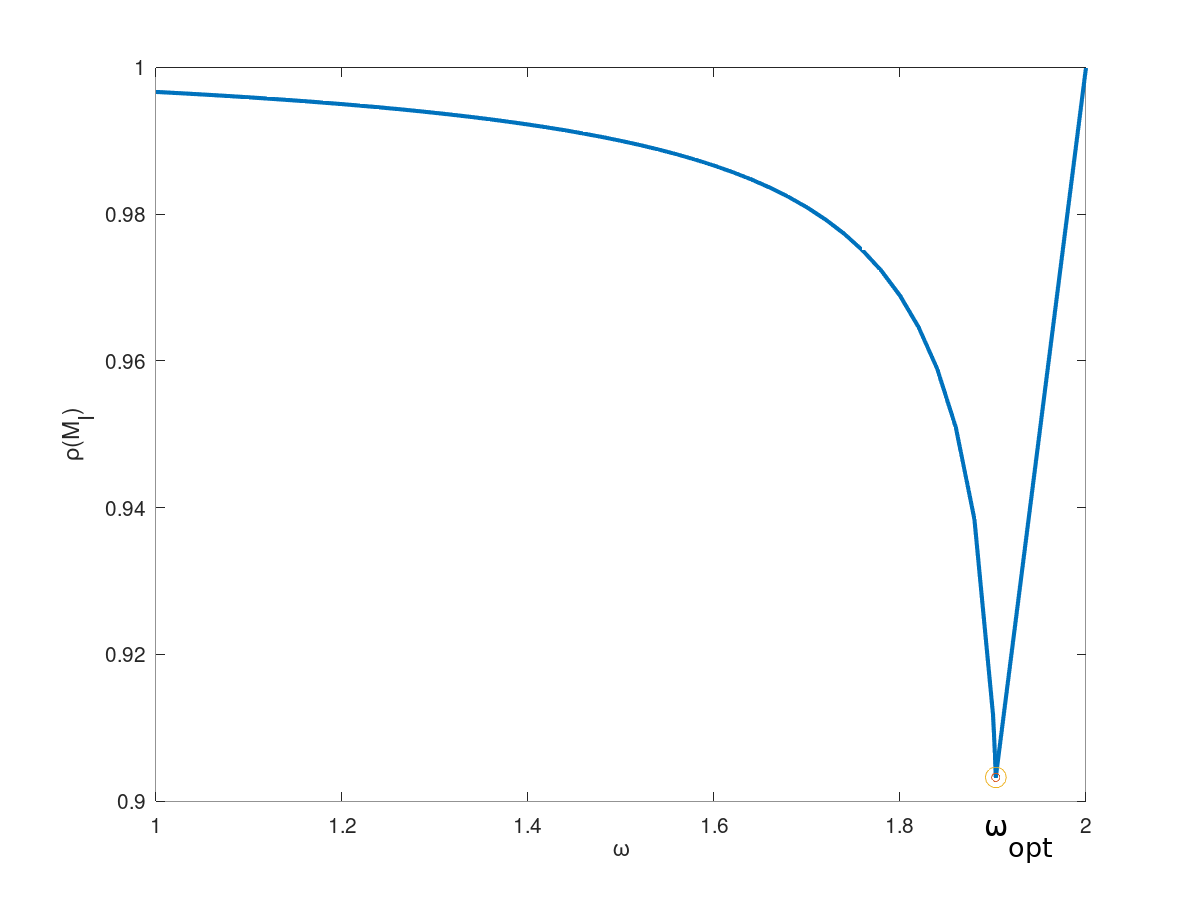
\includegraphics[width=0.4\linewidth]{omegaopt.png}
\caption{Comportamiento de $\rho(\Mb_\omega)$. Se ve que tiene un mínimo cerca de $\omega=1.904$ que se corresponde con un radio espectral cercano a $0.9$. }
\end{figure}

\section{Método de gradiente (o del descenso más rápido)}
Cuando trabajamos con matrices simétricas definidas positivas es posible reemplazar el problema:
$$
\mbox{(P1) Hallar $\xb\in \R^n$ tal que
}\,\Ab\xb=\bb
$$
por un problema de minimización  asociado a la función  $J:\Rn\to \R$, $J(\zb)=\frac{1}{2}\zb^T\Ab\zb-\zb^T\bb$:
$$
\mbox{(P2) Hallar $\xb\in \Rn$ tal que}\, J(\xb)=
\min_{\yb\in \R^n}J(\yb).
$$
En efecto, calculemos para $\xb\in \Rn$, $\zb\in \Rn, \zb\ne\cero$ y $t\in \R$ arbitrarios, la expresión
$$
h(t)=J(\xb+t\zb)= \frac{1}{2}(\xb+t\zb)^T\Ab(\xb+t\zb)-(\xb+t\zb)^T\bb,
$$
desarrollando los términos resulta
\begin{equation}
\label{eq:derideh}
h(t)=\frac{1}{2}t^2\zb^T\Ab\zb+t\left(\zb^T\Ab\xb-\zb^T\bb\right) +\frac{1}{2}\xb^T\Ab\xb-\xb^T\bb
\end{equation}
una cuadr\'atica en la variable $t$, con mínimo en
\begin{equation}
\label{eq:minsearch}
t_m=\frac{\zb^T\Ab\xb-\zb^T\bb}{\zb^T\Ab\zb}=\frac{\zb^T(\Ab\xb-\bb)}{\zb^T\Ab\zb}.
\end{equation}
\emph{Supongamos que $\xb$ resuelve (P1)}. En ese caso debe ser $t_m=0$ y entonces
$$
J(\xb)=h(0)\le h(t)=J(\xb+t\zb)
$$
para todo $t$ y vemos que
$$
J(\xb)=\min_{\yb\in\Rn}J(\yb),
$$
lo que dice que $\xb$ resuelve $(P2)$.
Recíprocamente: si $\xb$ es tal que
$$
J(\xb)=\min_{\yb\in\Rn}J(\yb),
$$
repetimos la cuenta anterior y vemos que el mínimo de $h(t)$ está en $t=0$ lo que dice que
$$0=\frac{\zb^T\Ab\xb-\zb^T\bb}{\zb^T\Ab\zb}
$$
es decir
$$
\zb^T(\Ab\xb-\bb)=0,
$$
para todo $\zb\neq \cero$, lo que indica que \footnote{Tomando, por ejemplo, $\zb=\Ab\xb-\bb$.}
$$
\Ab\xb-\bb=\cero,
$$
es decir
$$
\Ab\xb=\bb.
 $$
 y entonces $\xb$ resuelve $(P1)$.
\tcc
Ejemplo en $\R^2$: Consideremos la matriz $
\Mb=\begin{pmatrix}
     5&2\\
     2&4
    \end{pmatrix}
$ y el vector  $
\bb=\begin{pmatrix}
     1\\
     0
    \end{pmatrix}
$. El sistema asociado
$$
\Mb\xb=\bb,
$$
tiene por solución $\xb=\begin{pmatrix}
    1/4\\
    -1/8
     \end{pmatrix}.
$
Por otro lado,
$$
J(x_1,x_2)=5/2x_1^2+2x_2^2+2x_1x_2-x_1,
$$
y en la Figura \ref{fig:curvasdeJ} vemos las curvas de nivel de $J$ y el punto $\xb$ (en rojo) solución del sistema.
\etcc

\begin{figure}[h]
\centering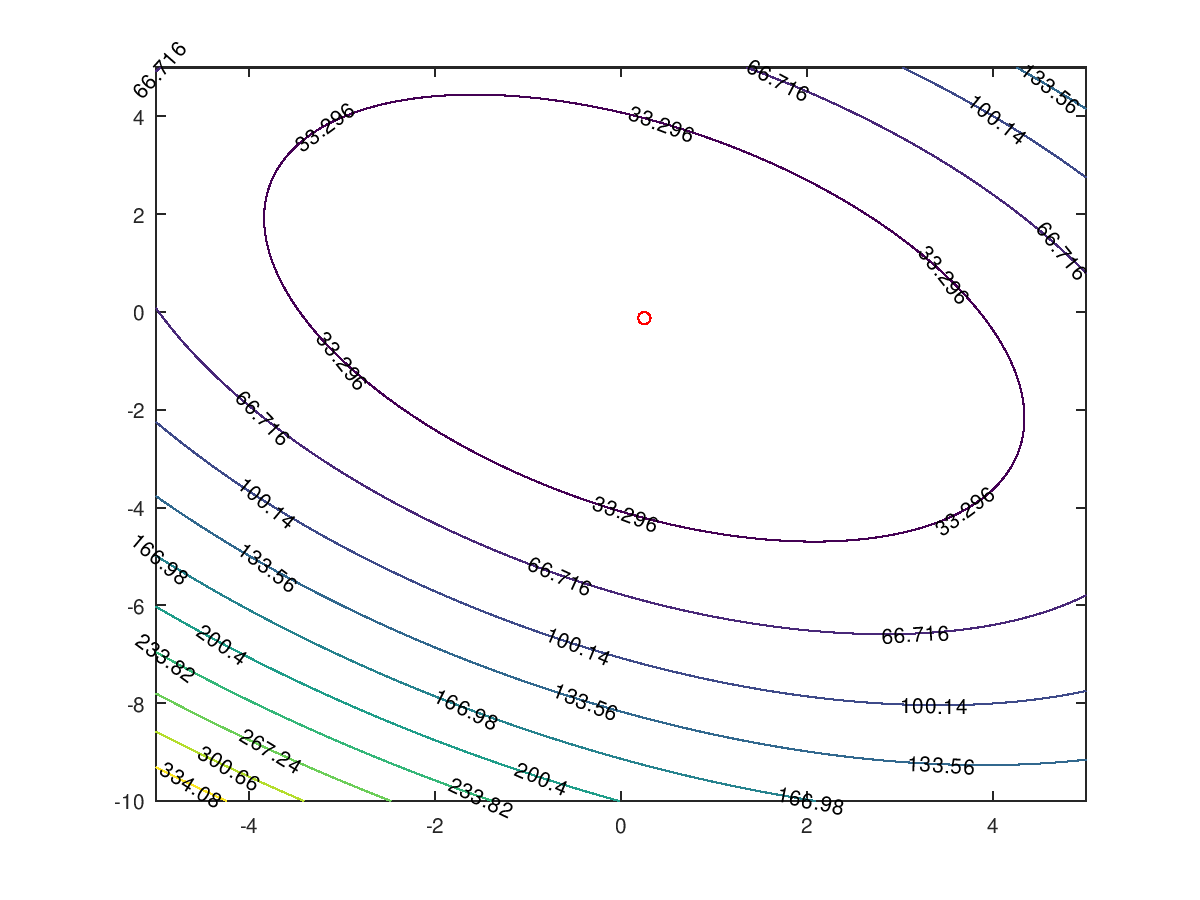
\includegraphics[width=0.4\linewidth]{curvasnivel.png}
\label{fig:curvasdeJ}
\caption{Curvas de nivel de $
J(x_1,x_2)=5/2x_1^2+2x_2^2+2x_1x_2-x_1
$.}
\end{figure}
\tcc
Antes de continuar observemos que tomando en \eqref{eq:derideh} , $\zb=\eb_i$ (el canónico $i$) se tiene que
$$\frac{\partial J(\xb)}{\partial x_i}=\lim_{t\to 0} \frac{J(\xb+t\eb_i)-J(\xb)}{t}=[\Ab\xb-\bb]_i,$$
donde el corchete representa la coordenada $i$ del vector $\Ab\xb-\bb$. En particular tenemos
$$
\nabla J(\xb)=\Ab\xb-\bb.
$$
\etcc
Lo que hemos visto indica que para resolver un sistema con una matriz SDP podemos alternativamente atacar un problema de minimización en $\Rn$. Para comenzar simplificando este nuevo problema vamos a intentar llevarlo a uno que sea iterativo en $\R$. Este es un m\'etodo de busqueda por líneas: dado $\xb_i$ elegimos una dirección de búsqueda $\zb_i$ y un escalar $\lambda_i$ tal que
$$
\xb_{i+1}=\xb_i+\lambda_i\zb_i.
$$
En un caso general quisieramos $\lambda_i$ tal que
$$
J(\xb_{i}+\lambda_i\zb_i )=\min_{t\in \R}J(\xb_i+t\zb_i),
$$
lo que nos llevaría a resolver
$$
0=\frac{dJ(\xb_{i}+t\zb_i )}{dt}|_{t=\lambda_i}=\nabla J(\xb_{i}+\lambda_i\zb_i )^T\zb_i.
$$
En el caso que nos interesa ya sabemos despejar $\lambda_i$ (ver \eqref{eq:minsearch}):
$$
\lambda_i=-\frac{\zb_i^T(\Ab\xb_i-\bb)}{\zb_i^T\Ab\zb_i}=
\frac{\zb_i^T\rb_i}{\zb_i^T\Ab\zb_i}
$$
donde $\rb_i=\bb-\Ab\xb_i$ es el residuo.

Este método no nos sugiere como elegir el vector de búsqueda $\zb_i$ en cada paso. Una forma natural es utilizar la dirección de mayor decrecimiento de la función $J$ en el punto $\xb_i$ : $-\nabla J(\xb_i)=\bb-\Ab\xb_i=\rb_i$. Esto da lugar al método del gradiente o del descenso más rápido:
$$
\xb_{i+1}=\xb_i+\frac{\rb_i^T\rb_i}{\rb_i^T\Ab\rb_i}
\rb_i.
$$
El proceso anterior puede converger muy lentamente. En cada paso minimizamos (de forma exacta en aritmética exacta) a lo largo de la recta $\xb_i+\lambda \zb_i$.

Una mejora sustancial sería comenzar en un $x_0$, minimizar a lo largo de una recta, luego a lo largo de un plano, e ir aumentando la dimensión. Por ejemplo podríamos  intentar minimizar el paso $i$ en
$$
J(\xb_{i+1})=\min_{\yb\in \langle \zb_0,\cdots\zb_i \rangle + x_0}J(\yb)
$$
que claramente daría un algoritmo que finaliza\footnote{Al menos en aritmética exacta.} en a lo sumo $n$ pasos. Obviamente, vemos que el problema que aparece es la dificultad de minimizar en dimensiones mayores a uno. Hay, sin embargo, un modo de lograr nuestro propósito minimizando sobre líneas, si es que elegimos las direcciones de búsqueda de modo adecuado. Este algoritmo lo estudiamos en la siguiente sección.
\section{Gradiente Conjugado}
Observemos, antes de continuar, que una matriz simétrica (o Hermitiana) definida positiva define un producto interno a través de la operación\footnote{Dejamos como ejercicio esta afirmación.}
$$
\xb^T\Ab\yb.
$$
En particular este producto posee la siguiente norma asociada
$$
\|\xb\|_A=\sqrt{\xb^T\Ab\xb}.
$$
Teniendo esta norma definida probamos lo siguiente.
\tcc
\begin{lema}
Supongamos que las direcciones de búsqueda son $\Ab$ ortogonales (i.e. $\zb_i^T\Ab\zb_j=0$) y en cada paso $\lambda_i$ se elige para minimizar sobre la línea correspondiente. Entonces
$$
\min_{\xb_i+\langle \zb_i\rangle}J(\yb)=J(\xb_{i+1})=\min_{\yb\in \xb_0+\langle \zb_0,\zb_1,\cdots,\zb_i \rangle} J(\yb)
$$
\end{lema}
\etcc
\begin{proof}
 Sea $W_{i+1}=\langle \zb_0,\zb_1,\cdots,\zb_i \rangle$ y tomo $\zb\in \xb_0+W_{i+1}$ arbitrario. Por construcción, se puede escribir
 $$\zb=\yb+t\zb_i$$ con $\yb\in \xb_0+ W_i=\xb_0+\langle \zb_0,\zb_1,\cdots,\zb_{i-1} \rangle$.

Observamos que
  $$
 \min_{\zb\in \xb_0+W_{i+1}}J(\zb)=\min_{\yb\in\xb_0+W_{i},t \in \R} J(\yb+t \zb_i)
 $$

Escribimos
$$
J(z)=J(\yb+t\zb_i)=\frac{1}{2}t^2\zb_i^T\Ab\zb_i+t\left(\zb_i^T\Ab\yb-\zb_i^T\bb\right) +\frac{1}{2}\yb^T\Ab\yb-\yb^T\bb
$$
pero, usando que $\zb_i^T\Ab\zb_j=0$
$$
\zb_i^T\Ab\yb=\zb_i^T\Ab\xb_0=\zb_i^T\Ab\xb_i
$$
$$
J(\yb+t\zb_i)=\left(\frac{1}{2}t^2\zb_i^T\Ab\zb_i+t\left(\zb_i^T\Ab\xb_i-\zb_i^T\bb\right)\right) +\frac{1}{2}\yb^T\Ab\yb-\yb^T\bb
$$
de donde resulta que
para minimizar en $\zb$ basta minimizar ambos términos: el primero en $t\in \R$ el segundo en $\yb\in W_i$. Pero el $t$ óptimo es justamente $\lambda=\frac{\zb_i^T\Ab\rb_i}{\zb_i^T\Ab\zb_i}$ provisto por nuestro método. En definitiva
  el resultado sale por inducción.
\end{proof}

\tccdefi
\begin{center}Las direcciones $\Ab$ ortogonales suelen llamarse conjugadas lo que da nombre al algoritmo que veremos mas adelante.
\end{center}
\etcc
Queremos un método que minimice sobre direcciones conjugadas (y no sea costoso)

Idea: A-ortogonalizar los residuos
\begin{itemize}
 \item $\zb_0=\rb_0$
 \item $\zb_i=\rb_i-\sum_{j=0}^{i-1}\frac{\zb_j^T\Ab\rb_i}{\zb_j^T\Ab\zb_j}\zb_j$
\end{itemize}



Vale lo siguiente
\begin{itemize}
 \item $\langle \zb_0, \zb_1\cdots ,\zb_i\rangle =\langle \rb_0, \rb_1\cdots ,
 \rb_i\rangle$
\item $\rb_i^T\rb_j=0$, pues $J(\xb_i+t\rb_j)$ tiene un mínimo en $t=0$, si $0\le j<i$. Luego derivando y evaluando en $t=0$
$$
0=\rb_j^T(\Ab\xb_i-\bb)=\rb_j^T\rb_i.
$$
\item Existe $m\le n$ tal que
$$
\xb_0\neq \xb_1\neq \cdots \neq \xb_m= \xb
$$
$$
W_{0}\subsetneq W_1\subsetneq \cdots \subsetneq W_m
$$

\item Para todo $1\le i\le m$, $\{ \zb_0,\zb_1\cdots \zb_{i-1}\}$ (resp. $\{ \rb_0,\rb_1\cdots \rb_{i-1}\}$) es una base $A$ ortogonal (resp. ortogonal) de $W_i$.
 \item $\zb_i^T\rb_i=\rb_i^T\rb_i$. Pues
 $\zb_i=\rb_i-\sum_{j=0}^{i-1}\frac{\zb_j^T\Ab\rb_i}{\zb_j^T\Ab\zb_j}\zb_j$ y entonces
 $$\rb_i^T\zb_i=\rb_i^T\rb_i-\sum_{j=0}^{i-1}\frac{\zb_j^T\Ab\rb_i}{\zb_j^T\Ab\zb_j}\rb_i^T\zb_j=\rb_i^T\rb_i$$
 pues para cada $j\le i-1$,
 $\zb_j\in W_i=\langle \rb_0,\cdots,\rb_{i-1}\rangle$, $\rb_i^T\zb_j=0.$
 \end{itemize}


 Queremos hallar las direcciones de búsqueda sin hacer Gram-Schmidt (o sea mas rápido)

Escribamos $\zb_i$ en la base de los residuos (ortogonales),
$$
\zb_i=\sum_{j=0}^{i}\frac{\zb_i^T\rb_j}{\rb_j^T\rb_j}\rb_j,
$$
ya vimos que
$\zb_i^T\rb_i=\rb_i^T\rb_i$
pero además
$\zb_i^T(\rb_i-\rb_l)=\zb_i^T\Ab(\xb_i-\xb_l)=0$ porque $\xb_i-\xb_l\in W_i$ y $\zb_i$ es $A$ ortogonal a $W_i$.
$$
\zb_i=\sum_{j=0}^{i}\frac{\zb_i^T\rb_j}{\rb_j^T\rb_j}\rb_j=\sum_{j=0}^{i}\frac{\rb_i^T\rb_i}{\rb_j^T\rb_j}\rb_j=\rb_i + \rb_i^T\rb_i\sum_{j=0}^{i-1}\frac{\rb_j}{\rb_j^T\rb_j},
$$
como la ultima sumatoria permite escribir recursivamente las direcciones de búsqueda

$$
\rb_i + \rb_i^T\rb_i\sum_{j=0}^{i-1}\frac{\rb_j}{\rb_j^T\rb_j}=\rb_i + \frac{\rb_i^T\rb_i}{\rb_{i-1}^T\rb_{i-1}}\left( \rb_{i-1}+\rb_{i-1}^T\rb_{i-1}\sum_{j=0}^{i-2}\frac{\rb_j}{\rb_j^T\rb_j}\right)
$$
entonces
$$
\zb_i=\rb_i+\frac{\rb_i^T\rb_i}{\rb_{i-1}^T\rb_{i-1}}\zb_{i-1}
$$
los residuos  pueden obtenerse de
$$\xb_{i+1}=\xb_i+\lambda \zb_i$$
$$
\rb_{i+1}=\rb_i+\lambda_i\Ab\zb_i
$$

Tomo $\xb_0$, calculo $\rb_0$ asigno $\zb_0=\rb_0$

\noindent { for i=0... }
\begin{itemize}
 \item $\lambda_i=\frac{\rb_i^T\rb_i}{\zb_{i}^T\Ab\zb_i}$
 \item $\xb_{i+1}=\xb_{i}+\lambda_i \zb_i$
 \item $\rb_{i+1}=\rb_i+\lambda_i\Ab\zb_i$
\item $
\zb_{i+1}=\rb_{i+1}+\frac{\rb_{i+1}^T\rb_{i+1}}{\rb_{i}^T\rb_{i}}\zb_{i}
$

\end{itemize}
end

Aplicado a nuestro caso de ejemplo: para un error de orden $10^{-4}$ tarda $0.057$ segundos...
\section{GC y aproximación polinomial}
Para estudiar el error del GC notemos
$$
W_i=\langle \rb_0, \Ab\rb_0, \cdots \Ab^{i-1}\rb_0\rangle
$$
lo cual se ve por inducción. Si $i=1$ es cierto, y asumiendo que vale para $i$ queremos ver que vale para $i+1$. Para eso vemos que basta con ver que
$$
W_{i+1}\subset
\langle \rb_0, \Ab\rb_0, \cdots \Ab^{i}\rb_0\rangle
$$
puesto que $dim(W_{i+1})=i+1$

Asumiendo entonces que
$$W_{i}\ni \rb_{i-1},\zb_{i-1}\in \langle \rb_0, \Ab\rb_0, \cdots ,\Ab^{i-1}\rb_0\rangle$$



se tiene que  $\rb_{i}=\rb_{i-1}-\lambda_{i-1}\Ab\zb_{i-1}\in \langle \rb_0, \Ab\rb_0, \cdots ,\Ab^{i}\rb_0\rangle$
que es lo que queríamos ver.

En general, dada una matriz $\Ab$, subespacios de la forma
$\langle \bb, \Ab\bb, \cdots ,\Ab^{i}\bb\rangle$, se llaman subespacios
de Krylov. La identidad de abajo permite relacionar esos subespacios con polinomios.
$$\langle \rb_0, \Ab\rb_0, \cdots \Ab^{i-1}\rb_0\rangle=\{ p(\Ab)\rb_0: p\in P_{i-1}[x]\}=$$
$$=\{ q(\Ab)(\xb-\xb_0): q\in P_{i}[x],\ q(0)=0\}$$

Va a resultar cómodo estudiar el error en la norma $\|\cdot\|_A$: es decir,  acotar
$$
\|\xb-\xb_i\|_{A}$$
Como $\rb_i$ es ortogonal a $W_i$, $\xb-\xb_i
$ es $A$ ortogonal a $W_i$
$$
\|\xb-\xb_i\|_{A}=\inf_{\yb\in W_i}\|\xb-\xb_i-\yb\|_{A}
$$
como $\xb_0-\xb_i\in W_i$
$$
\|\xb-\xb_i\|_{A}=\inf_{\yb\in W_i}
\|\xb-\xb_0-\yb\|_{A}
=$$

$$
=\inf_{q\in P_{i}[x],q(0)=0}\|\xb-\xb_0-q(\Ab)(\xb-\xb_0)\|_{A}
=$$
$$
=\inf_{p\in P_i[x],p(0)=1}\|p(\Ab)(\xb-\xb_0)\|_{A}
\le$$
$$
\inf_{p\in P_i[x],p(0)=1}\|p(\Ab)\|_{A}\|(\xb-\xb_0)\|_{A}
$$

pero
$$
\|p(\Ab)\|_A^2=\sup_{\xb\neq\cero}\frac{\|p(\Ab)\xb\|_A^2}{\|\xb\|_A^2}=
$$
$$=\sup_{\xb\neq\cero}\frac{(p(\Ab)\xb)^T\Ab (p(\Ab)\xb)}{\xb^T\Ab\xb}=\sup_{\xb\neq\cero}\frac{\xb^T p(\Ab)^T\Ab p(\Ab)\xb}{\xb^T\Ab\xb}=
$$
$$
=\sup_{\xb\neq\cero}\frac{\xb^T\Ab^{1/2} p(\Ab)^T p(\Ab)\Ab^{1/2}\xb}{\xb^T\Ab^{1/2}\Ab^{1/2}\xb}=sup_{\yb\neq\cero}\frac{\yb^T p(\Ab)^T p(\Ab)\yb}{\yb^T\yb}
=$$
$$
=sup_{\yb\neq\cero}\frac{ \|p(\Ab)\yb\|_2^2}{\|\yb\|^2_2}
=\|p(\Ab)\|_2^2=\rho(p(\Ab))^2\le \max_{\lambda\in [\lambda_1,\lambda_n]}p(\lambda)^2$$

En definitiva

$$
\|p(\Ab)\|_A\le  \max_{x\in [\lambda_1,\lambda_n]}|p(x)|
$$
y hay que acotar
$$
\inf_{p\in P_i[x],p(0)=1}\max_{x\in [\lambda_1,\lambda_n]}|p(x)|
$$
esto, por suerte, lo estudió Chebyshev.

En el intervalo $[-1,1]$ los polinomios de Chebyshev son
$$
T_0(x)=1,T_1(x)=x,T_2(x)=2x^2-1,\cdots
$$
en general
$$
T_{n+1}(x)=2T_{n}(x)-T_{n-1}(x)
$$

Para $x\in [-1,1]$, $|T_n(x)|\le 1$

(de hecho
en ese rango $T_n(x)=\cos(n\cos^{-1}(x))$)

para $|x|\ge 1$
$$
T_n(x)=\frac12\left((x+\sqrt{x^2-1})^n+ (x-\sqrt{x^2-1})^n\right)
$$


El polinomio $p(x)\in P_n[x]$ que minimimiza $\max_{x\in [\lambda_1,\lambda_n]}|p(x)|$ con la condición $p(0)=1$ es
$$
\frac{1}{T_n(\frac{\lambda_n+\lambda_1}{\lambda_1-\lambda_n})}T_n\left(\frac{2x-\lambda_n-\lambda_1}{\lambda_n-\lambda_1}\right)$$


$$
\inf_{p\in P_i[x],p(0)=1}\max_{x\in [\lambda_1,\lambda_n]}|p(x)|
\le \frac{2}{\left( \frac{\sqrt{\frac{\lambda_n}{\lambda_1}}+1}{\sqrt{\frac{\lambda_n}{\lambda_1}}-1}\right)^i+\left( \frac{\sqrt{\frac{\lambda_n}{\lambda_1}}-1}{\sqrt{\frac{\lambda_n}{\lambda_1}}+1}\right)^i}$$
es decir
$$
\inf_{p\in P_i[x],p(0)=1}\max_{x\in [\lambda_1,\lambda_n]}|p(x)|
\le 2\left(\frac{\sqrt{\kappa(\Ab)}-1}{\sqrt{\kappa(\Ab)}+1}\right)^i
$$

$$\|\xb-\xb_i\|_{A}\le 2\left(\frac{\sqrt{\kappa(\Ab)}-1}{\sqrt{\kappa(\Ab)}+1}\right)^i\|\xb-\xb_0\|_{A}$$


